\subsection{Hivents} % (fold)
\label{sec:hivents}
\subsubsection{General} % (fold)
\label{sub:general}
Hivents mean ``Historical Events''. They are the way historical events are defined and presented. They are stored in a database, and have attributes such as name, location, start- and endyear, description and associated media.
They are one of the most important concepts to visualize history in HistoGlobe.

% subsection general (end)
\subsubsection{Behavior} % (fold)
\label{sub:behaviour}
Hivents are represented on several locations in the UI, with the map, the Hivent-List and the Timeline being the most important ones.
Since usually more than one Hivent is being shown, it's important to signify the representation between one Hivent in different UI-Elements.
The main interface events to which the feedback occurs are mouse hovering and clicking, which leads to the Hivent being highlighted in all UI-elements.

  \begin{figure}[here]
\begin{center}
  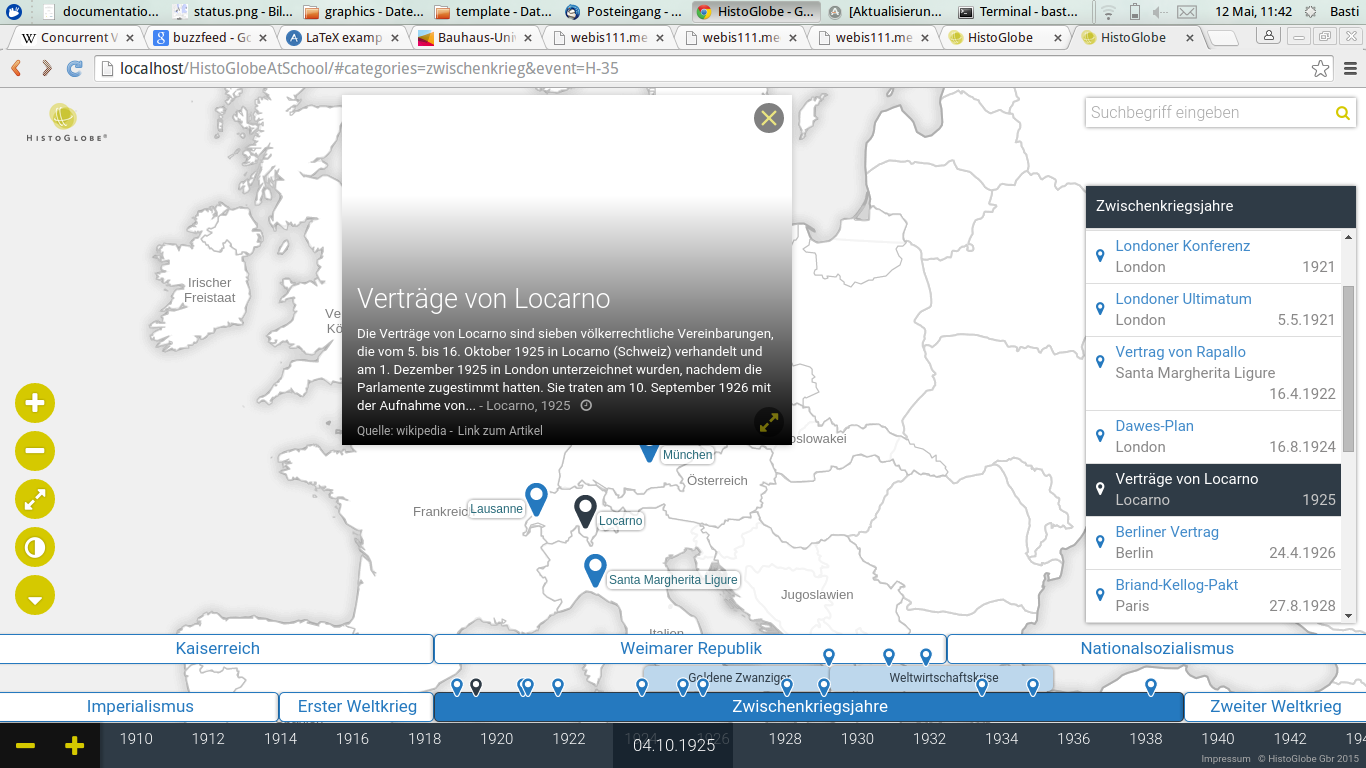
\includegraphics[width=0.8\textwidth]{graphics/activated_hivent.png}
  \end{center}

  \caption{Activated Hivent}
  \label{fig:activated_hivent}
\end{figure}

Upon being clicked on, it changes its status to active. An active Hivent gets focused in the map, it's marker are highlighted, it gets tagged in the URL bar and the Hivent box opens.

\subsubsection{Labels on Map}
Hivents on the Map were only represented by a marker.
Upon being very close they get automatically clustered.

The teacher demanded more information, so we attached labels to the Hivent markers.
We tried a Leaflet addon, but it didn't match our expectations of modifiability.
To do labels our own, we used how the markers were implemented in the first space. They are Leaflet DivIcons so they are a div with a background image essentially. To accomplish easily modifiable labels we simply added another div element.

In the first implementation the Hivents name was shown, but we realized this isn't appropriate on a map, so we switched to show the Hivents location. With this solution we got easily modifiable small weight labels.

To adjust them to reasonable readability we had to fulfill special requirements.
We needed an algorithm which was  particularly lightweight, since we can't precompute the labels positioning and due to the fact that we wanted to use \HG on school pcs and mobile devices.
Our solution is done by checking for an overlap by comparing the divs Bounding Boxes and moving the left label to the left on overlap.

On high zoom levels the amount of labels was so high the map wasn't readable anymore, so we remove them from a certain zoom level on.

  \begin{figure}[H]
\begin{center}
  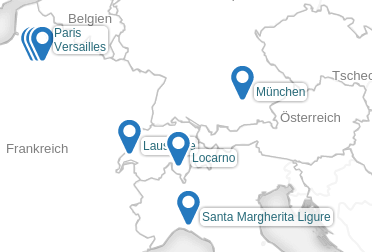
\includegraphics[width=0.8\textwidth]{graphics/overlapping_labels_2.png}
  \end{center}

  \caption{Overlapping labels}
  \label{fig:overlapping_labels}
  \end{figure}

\subsubsection{Hivent Regions}
A lot of historical events took place over a region, such as wars, so we wanted a region representation of hivents on the map.
We implemented an additional type of map marker to do this.
We added an additional optional attribute to the hivents, containing the polygon representing the region.
The implementation was done using Leaflets Polygon drawing capabilites.

  \begin{figure}[H]
\begin{center}
  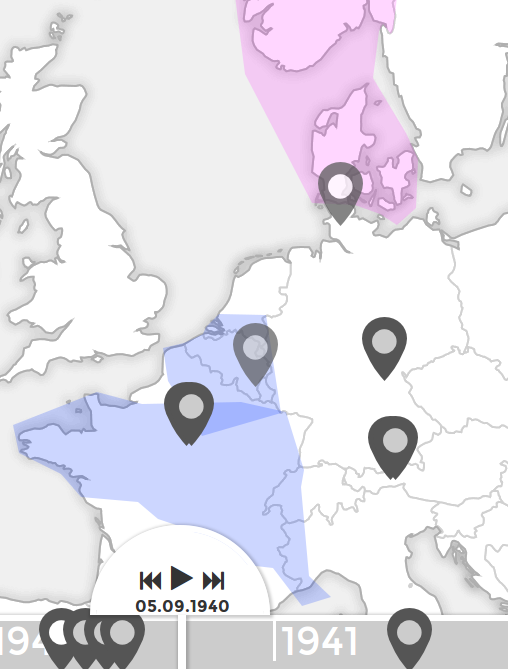
\includegraphics[width=0.3\textwidth]{graphics/status2.png}
  \end{center}

  \caption{Hivent regions with highlights}
  \label{fig:hivent_region_highlight}
  \end{figure}

As seen in \ref{fig:hivent_region_highlight}. 




% subsection hghghg (end)
% section section_name (end)

% subsection behaviour (end)
% section hivents (end)
